\documentclass[12pt,letterpaper]{article}
\usepackage[utf8]{inputenc}
\usepackage[spanish, es-tabla]{babel}
\usepackage[version=3]{mhchem}
\usepackage[journal=jacs]{chemstyle}
\usepackage{amsmath}
\usepackage{amsfonts}
\usepackage{amssymb}
\usepackage{makeidx}
\usepackage{graphicx}
\usepackage{xcolor}
\usepackage[stable]{footmisc}
\usepackage[section]{placeins}
%Paquetes necesarios para tablas
\usepackage{longtable}
\usepackage{array}
\usepackage{xtab}
\usepackage{floatrow}
\usepackage{multirow}
\usepackage{colortab}
\usepackage{caption}
\usepackage{enumitem}
%Paquete para el manejo de las unidades
\usepackage{siunitx}
\sisetup{mode=text, output-decimal-marker = {,}, per-mode = symbol, qualifier-mode = phrase, qualifier-phrase = { de }, list-units = brackets, range-units = brackets, range-phrase = --}
\usepackage{cancel}
%Paquetes necesarios para imágenes, pies de página, etc.

\usepackage{listings}
\usepackage{color}

\definecolor{dkgreen}{rgb}{0,0.6,0}
\definecolor{gray}{rgb}{0.5,0.5,0.5}
\definecolor{mauve}{rgb}{0.58,0,0.82}

\lstset{frame=tb,
  language=Java,
  aboveskip=3mm,
  belowskip=3mm,
  showstringspaces=false,
  columns=flexible,
  basicstyle={\small\ttfamily},
  numbers=none,
  numberstyle=\tiny\color{gray},
  keywordstyle=\color{blue},
  commentstyle=\color{dkgreen},
  stringstyle=\color{mauve},
  breaklines=true,
  breakatwhitespace=true,
  tabsize=3
}

%Instrucción para evitar la indentación
%\setlength\parindent{0pt}
%Paquete para incluir la bibliografía
\usepackage[backend=bibtex,style=chem-acs,biblabel=dot]{biblatex}
\addbibresource{references.bib}


%Modificación del formato de los captions
\usepackage[margin=10pt,labelfont=bf]{caption}

%Paquete para incluir comentarios
\usepackage{todonotes}

%Paquete para incluir hipervínculos
\usepackage[colorlinks=true, 
            linkcolor = blue,
            urlcolor  = blue,
            citecolor = black,
            anchorcolor = blue]{hyperref}

\begin{document}
\renewcommand{\labelitemi}{$\checkmark$}

\renewcommand{\CancelColor}{\color{red}}

\newcolumntype{L}[1]{>{\raggedright\let\newline\\\arraybackslash}m{#1}}

\newcolumntype{C}[1]{>{\centering\let\newline\\\arraybackslash}m{#1}}

\newcolumntype{R}[1]{>{\raggedleft\let\newline\\\arraybackslash}m{#1}}


\begin{center}

	\textbf{\LARGE{SIMULACIÓN DE MODELOS  DINÁMICOS BIOLÓGICOS}}\\
	\vspace{7mm}
	\textbf{\large{Realizado Por: Michael Santiago Díaz 160002613}}\\
	\textbf{\large{Entregado A: Ph.D Ángel Cruz}}\\
	\vspace{5mm}
	\textbf{\large{Universidad de los llanos}}\\
	\today
\end{center}



\section{Introducción }

Tutorial realizado con el fin de crear diagramas de modelos más complejos para ser analizados: 
\begin{itemize}
	\item modelo neuronal (Fitzhugh - Naguno)
	\item modelo de evolución del virus del sida
	\item modelo presa depredador (Lotka-Volterra)
\end{itemize}




\section{Modelo Neuronal de Fitzhugh - Naguno}


el modelo neuronal de Fitzhugh - Nagumo, describe el comportamiento de celulas nerviosas en condiciones ideales de laboratorio, se explica caracteristicas basicas de esta y  la funcion de una neurona por ejemplo, se tendria claro para representar este modelo de simulacion un adyacente que seria un modelo de simulacion que se pueda representar esquematicamente, claro esta que se explica lastrespartes inportantes de las neuronas:  las dendritas actuan como antenas que reciben los contactos de otras celulas,  en el soma se lleva a cabo la integracion de toda la informacion obtenida en las dendritas y finalmente el axon transmite a otras celulas el mensaje resultante de la integracion, se explica bastante bien las variables que inciden en el sistema, las dendritas se asocian al potencial que retienen x1 y x2 indican la influencia de x sobre su tasa de cambio y son constantes y E mide la corriente electrica actual a la que se encuentra sometida la neurona .\\

\begin{figure}
\centering
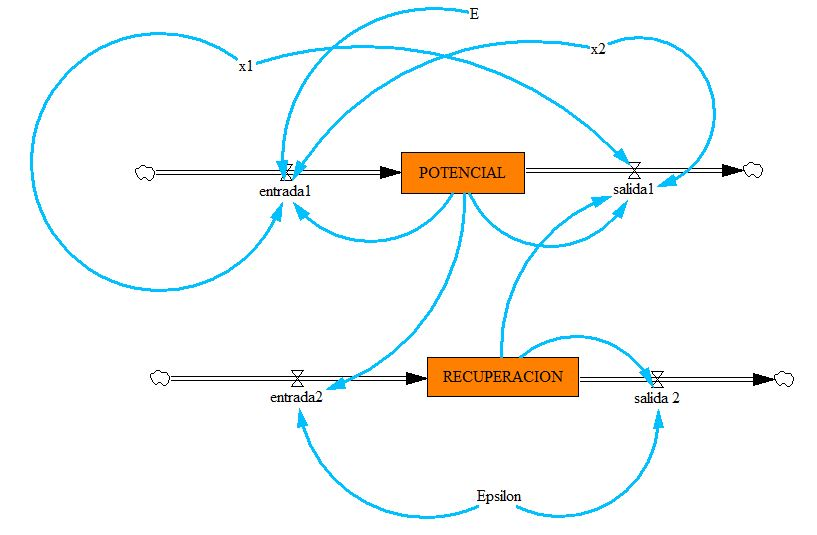
\includegraphics[width=5cm, height=5cm]{1.JPG}
\caption{\label{fig: } Modelo Neuronal }
\end{figure}

\begin{figure}
\centering
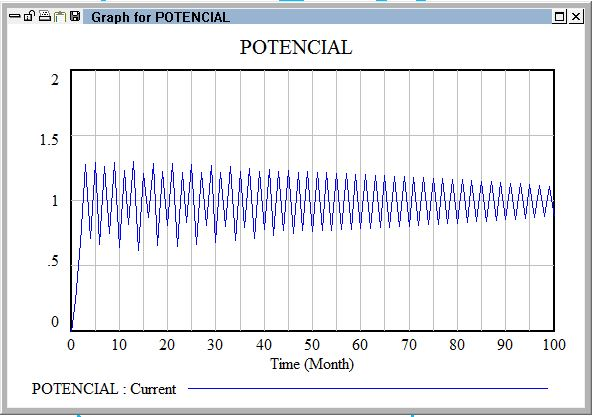
\includegraphics[width=5cm, height=5cm]{2.JPG}
\caption{\label{fig: }  Respuesta del Modelo Neuronal }
\end{figure}

\section{Modelo que estudia la respuesta inmunológica}


\subsection{Sistema inmunológico sano}

Entonces el proceso inmunológico funciona de la siguiente manera: un virus entra al cuerpo, que puede ser la gripe que entra por la nariz. Si otro virus entra por la sangre, el sistema inmunológico está siempre alerta para detectar y atacar al agente infeccioso antes de que cause daño. El que gente que sea el sistema inmunológico lo reconoce como un cuerpo ajeno, a estos se le llaman antígenos, y los antígenos deben ser eliminados.
La primera línea de defensa del cuerpo son los globulos blancos, estos circulan por la corriente sanguínea y en los tejidos del cuerpo, vigilantes de los antígenos.
Cuando un invasor entra, un glóbulo blanco rápidamente lo detecta y lo captura dentro de la célula. Enzimas en el interior del glóbulo blanco destruyen al antígeno procesándolo en pedacitos. A veces este proceso por sí solo es suficiente para eliminar al invasor. Sin embargo, en la mayoría de los casos, otras células del sistema inmunológico deben unirse a la lucha, otros tipos de glóbulos blancos, los linfocitos (que se tragan las células) y las células asesinas por naturaleza (células citotóxicas), y destruyen al microorganismo infeccioso.\\
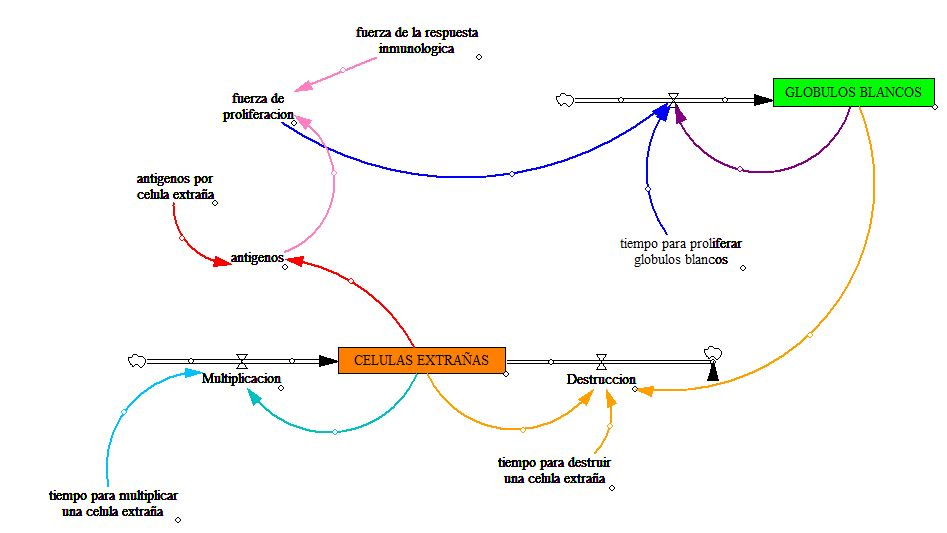
\includegraphics[width=10cm, height=5cm]{3.JPG}
\begin{figure}
\centering

\caption{\label{fig:3 } Modelo inmunologico}
\end{figure}
\\

\begin{figure}
\centering
\begin{minipage}{.5\textwidth}
  \centering
  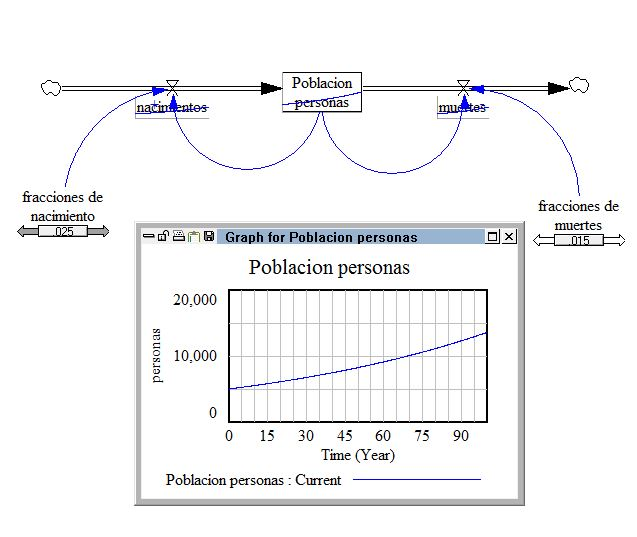
\includegraphics[width=1\linewidth]{4.jpg}
  \label{fig:test1}
\end{minipage}%
\begin{minipage}{.5\textwidth}
  \centering
  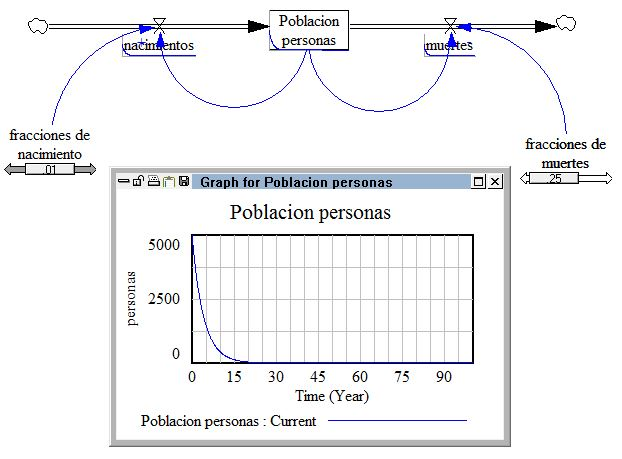
\includegraphics[width=.7\linewidth]{5.jpg}
  \label{fig:test2}
\end{minipage}
\end{figure}



\subsection{El modelo de Lotka-Volterra }
Se parte delas siguientes hipótesis:\\
\begin{itemize}

\item La especie depredadora se alimenta solo de la especie presa, mientras que ésta se nutre de un recurso que se encuentra en el hábitat en grandes cantidades.
\item Las dos poblaciones eran homogéneas, es decir, los parámetros de edad y sexo no cuentan.
\item  Las características son las mismas en todo el hábitat.
\item La probabilidad de interacción entre ambas especies es la misma.
\item Por lo que solo existen dos variables: el tamaño poblacional de la especie depredadora y el de la especie presa, que dependen únicamente del tiempo.
\end{itemize}
se representan la razón de nacimiento y muerte entre ambas especies, y les entran constantes que reflejan su interacción, beneficiosa para los depredadores, perjudicial para las presas. entonces se concluyoque  formuló que el cambio de los tamaños poblacionales de ambas especies son periódicos y el periodo depende solamente de la tasa de nacimiento de cada especie y la tasa de muerte de cada especie del tamaño inicial de las dos especies.\\\\

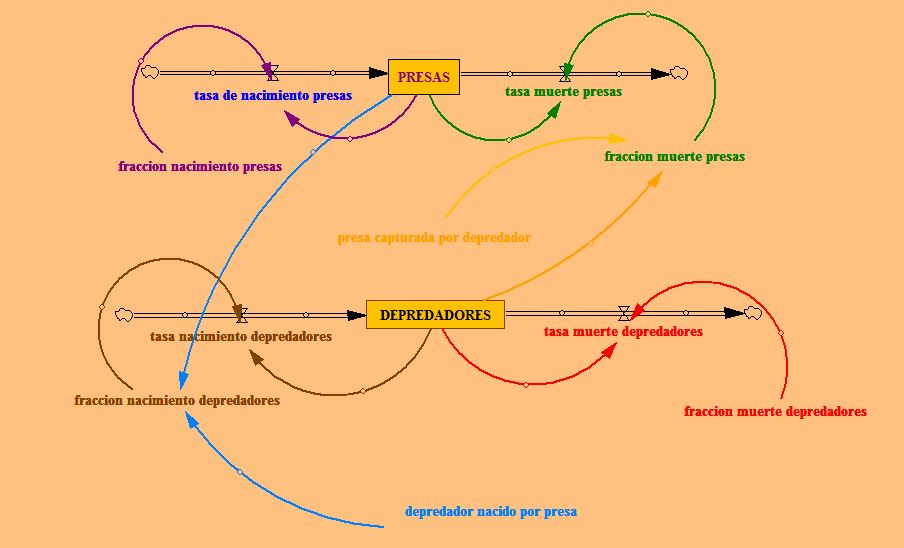
\includegraphics[width=12cm, height=8cm]{6.JPG}
\\\\\\\\\

\section{Conclusiones}
	Vensim es una gran herramienta que permite abstraer modelos complejos del mundo real, con los tres modelos realizados se demuestran las capacidades del programa.


\end{document}   